\subsubsection{Gerätefunktion}
\label{sec:geraetefunktion}

Ein gemessenes Spektrum kann als Faltung von Geräte- und Probenfunktion interpretiert werden. 
Aufgrund der hohen Kristallinität von Kochsalz kann hier jedoch der Anteil der Probe an der halbwertsbreite der Peaks vernachlässigt werden. Daraus folgt, dass die Halbwertsbreitenfunktion in etwa der Gerätefunktion entspricht. Die Halbwertsbreitenfunktion ist gegeben durch:
\begin{equation}
    FWHM(\Theta) = \sqrt{U \cdot \tan^2(\Theta) + V \cdot \tan(\Theta) + W}
\end{equation}
Mithilfe von scipy.optimize.curve\_fit können nun die Parameter $U, V, W$ bestimmt werden. Die Messwerte werden aus Tabelle~\ref{tab:peaks} übernommen. Für die Fitparameter ergibt sich:
\begin{equation*}
    U = \num{84,3(0,5)e-3}, \qquad V = \num{-0,5(0,8)e-3}, \qquad W = \num{90,0(0,3)e-3}
\end{equation*}
Messwerte und Fit sind in Abbildung~\ref{fig:geraetefunktion} dargestellt.

\begin{figure}[hbt!]
    \centering
    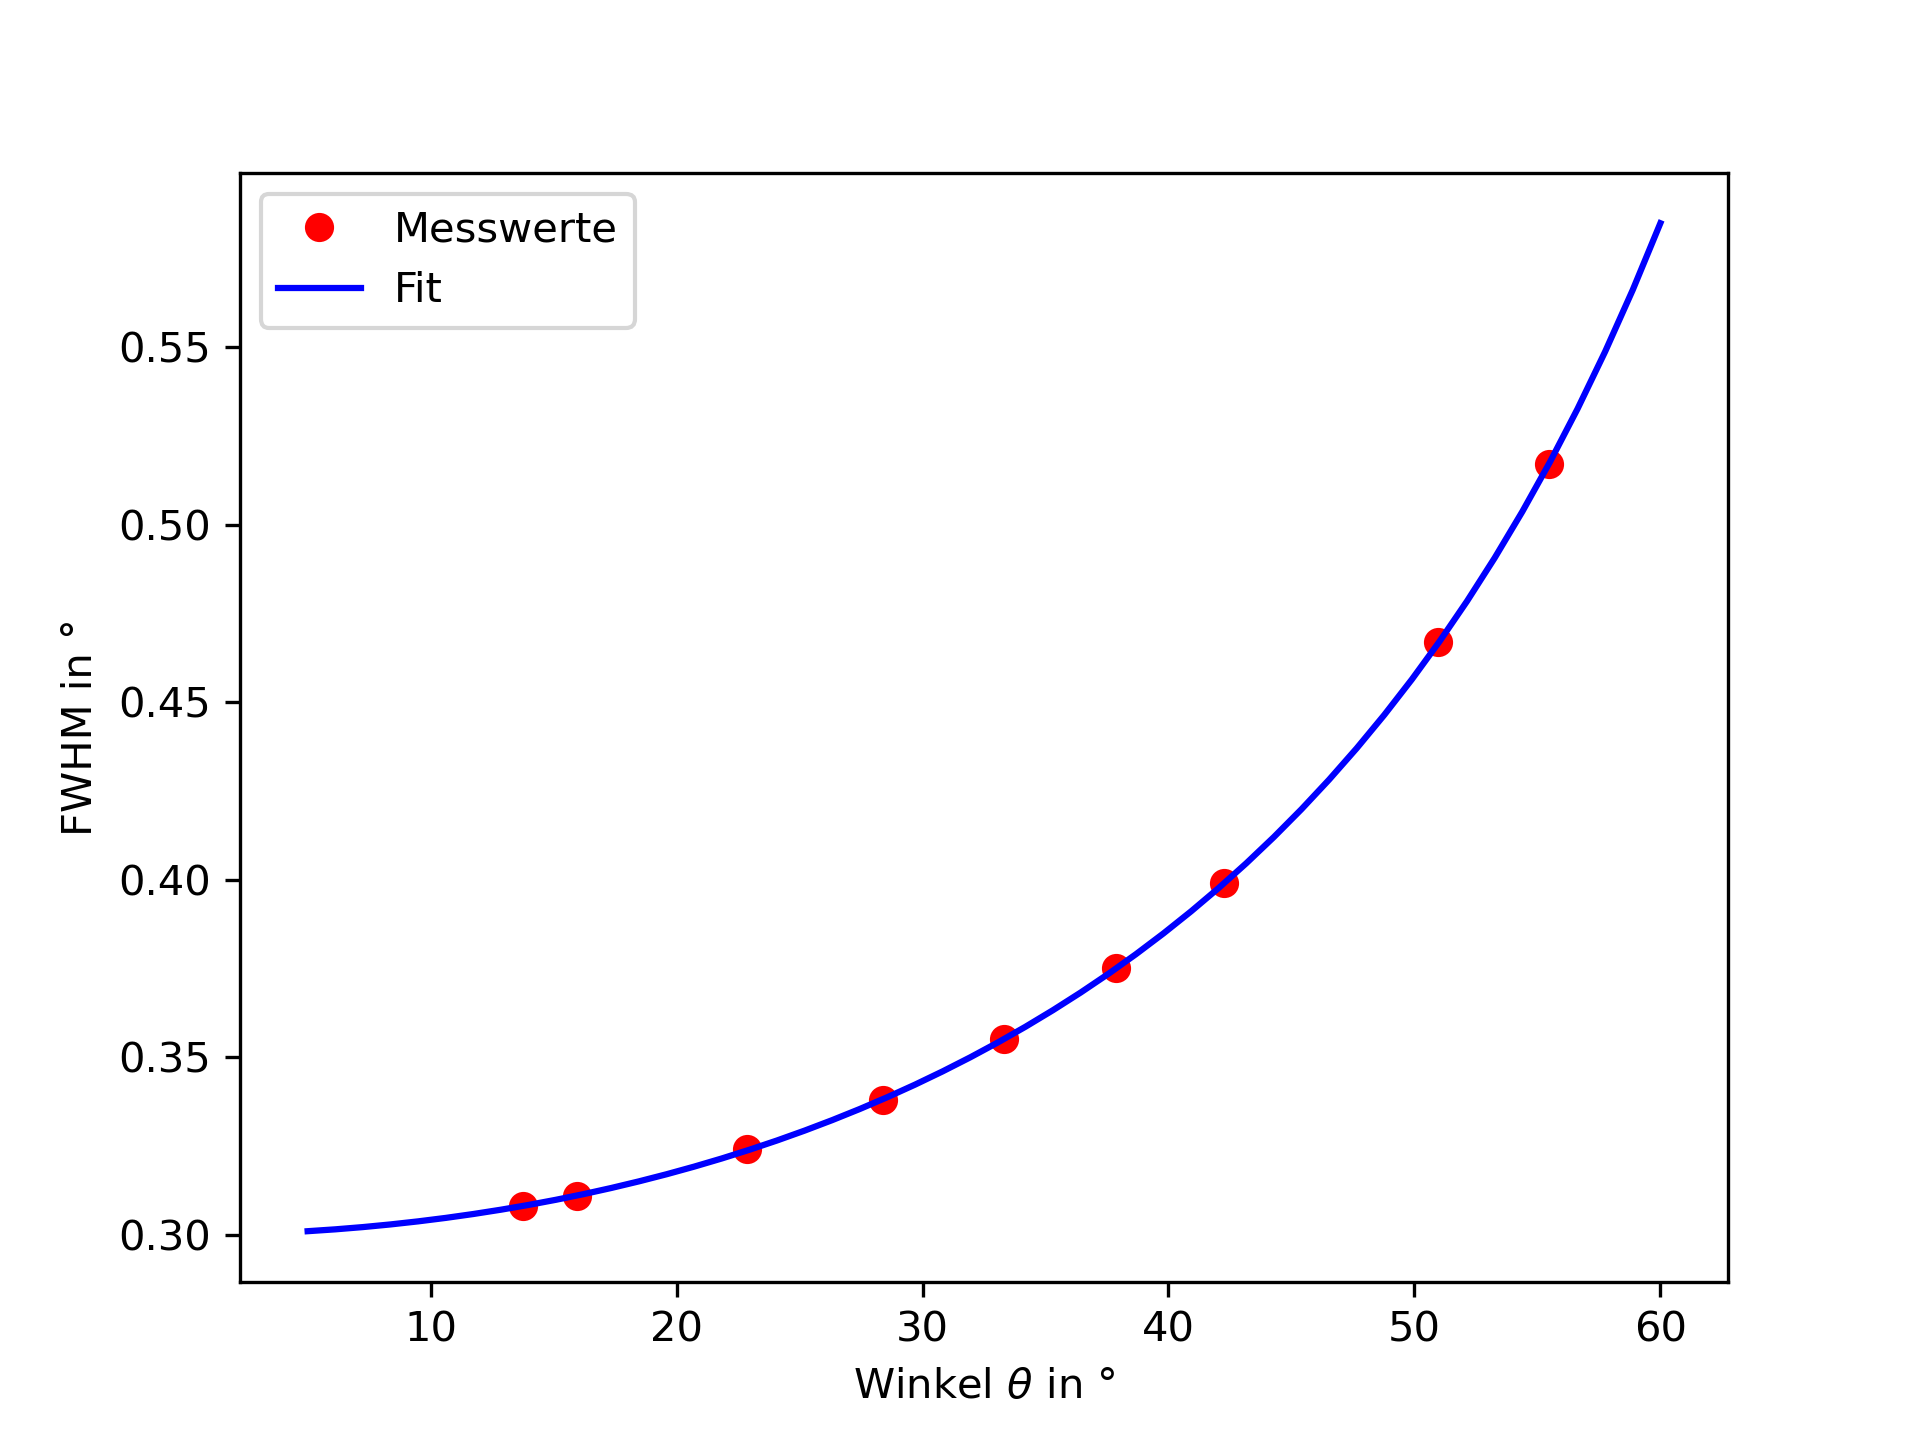
\includegraphics[width=0.7\textwidth]{fwhm_fit.png}
    \caption{Halbwertsbreite als Funktion des Streuwinkels mit den Messwerten in Rot und dem Fit in blau.}
    \label{fig:geraetefunktion}
\end{figure}

In der hier gemessenen Gerätefunktion lässt sich kein wirkliches Minimum feststellen. Ein Minimum stände hierbei für den Punkt der geringsten Streuung am Detektor, was für die genauesten Messwerte stände.


\subsubsection{Beurteilung der Messung}
Insgesamt können wir mit der Messung zufrieden sein. Die Peaks sind gut zu erkennen und die berechnete Gitterkonstante liegt nah am Literaturwert. Die Peaks sind jedoch nicht so scharf wie in der Theorie, was auf eine gewisse Unschärfe des Detektors zurückzuführen ist. Auch der Fit der Jana2020 Software hat gut funktioniert. Der Großteil der erkennbaren Peaks konnte gut gefittet werden, was ebenso auf eine funktionerende Messung schließen lässt. Mit den gewonnenen Werten konnte auch ein gutes Modell für den Aufbau des NaCl-Kristalls bestätigt werden.\\
Bei zukünftigen Messungen könnte leicht die Genauigkeit bzw. das Signal-Rausch-Verhältnis erhöht werden, indem die Messzeit verlängert wird. Auch eine bessere Justierung des Detektors könnte die Messung verbessern. Für die Erfassung von mehr Peaks könnte ebenso der Winkelbereich vergrößert werden.
\clearpage
